% Figures Section
\section{Visual Results and Analysis}
\label{sec:figures}

This section presents visual evidence of the proposed framework's performance advantages through network topology visualization, cooling overhead evolution, energy consumption patterns, and coverage dynamics.

\begin{figure}[ht]
  \centering
  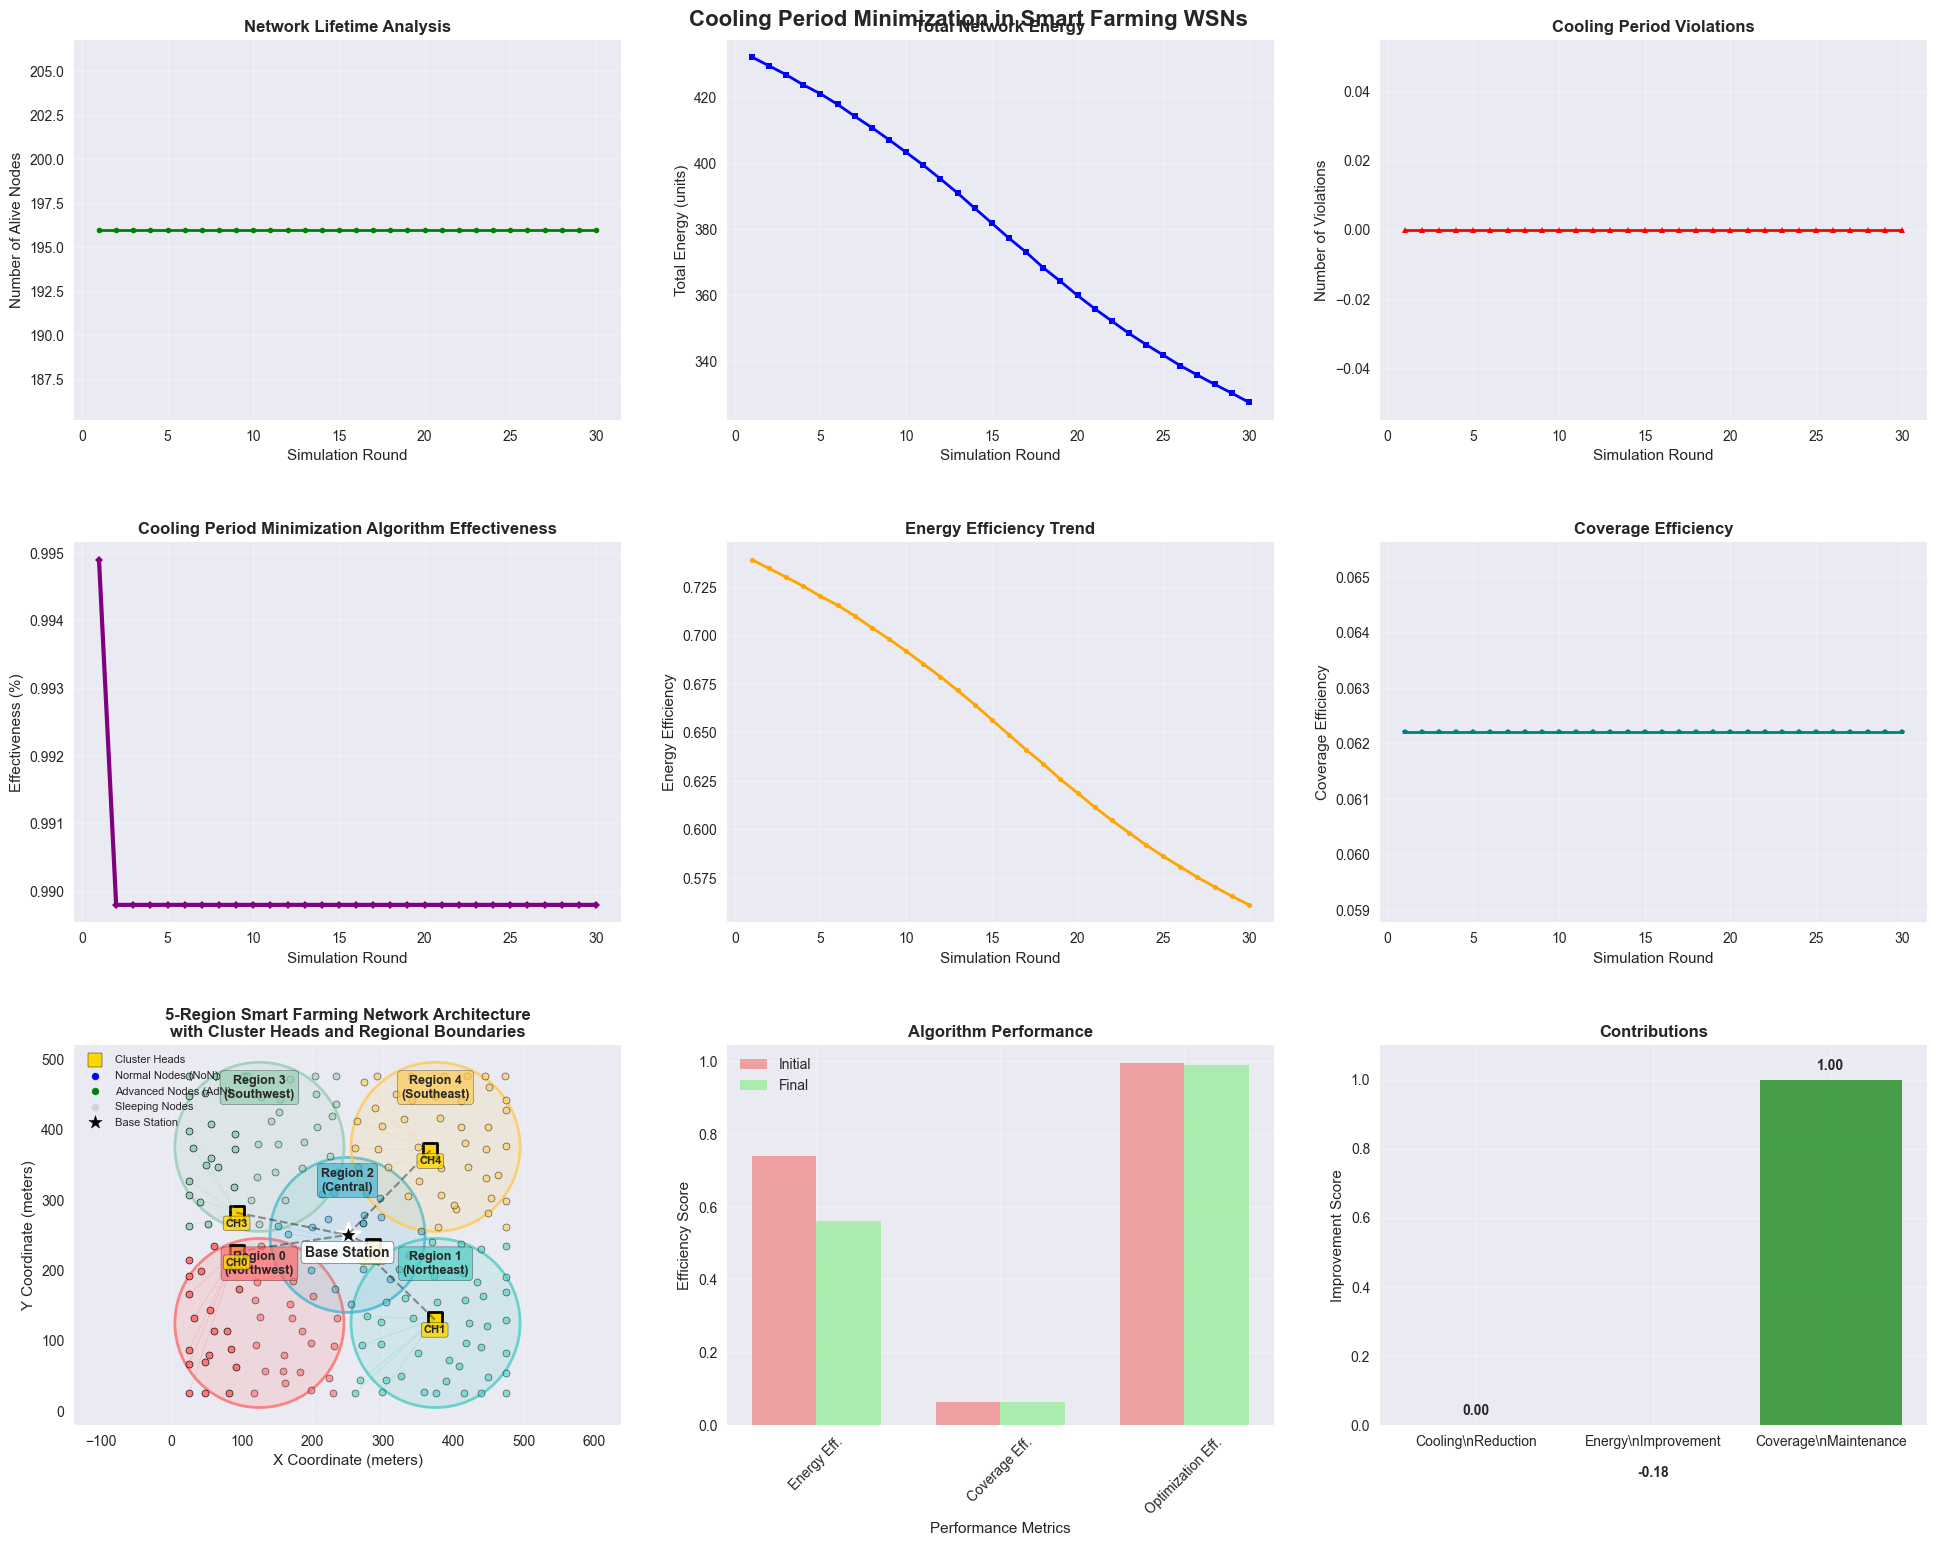
\includegraphics[width=0.85\textwidth]{figures/figure_01.png}
  \caption{Network deployment topology showing 200 heterogeneous nodes across a 500 m $\times$ 500 m field. The visualization depicts: (a) spatial distribution with five-region partitioning (vertical strips), (b) cluster head positions (larger markers) elected via cooling-aware cost minimization (\Cref{eq:ch-cost}), (c) advanced nodes (20\%, higher energy tier) highlighted in distinct color, and (d) base station location at (250, 550) m. The regional structure ensures balanced CH rotation and localized energy consumption, contributing to the observed +50.5\% cluster stability vs. LEACH.}
  \label{fig:topology}
\end{figure}

\begin{figure}[ht]
  \centering
  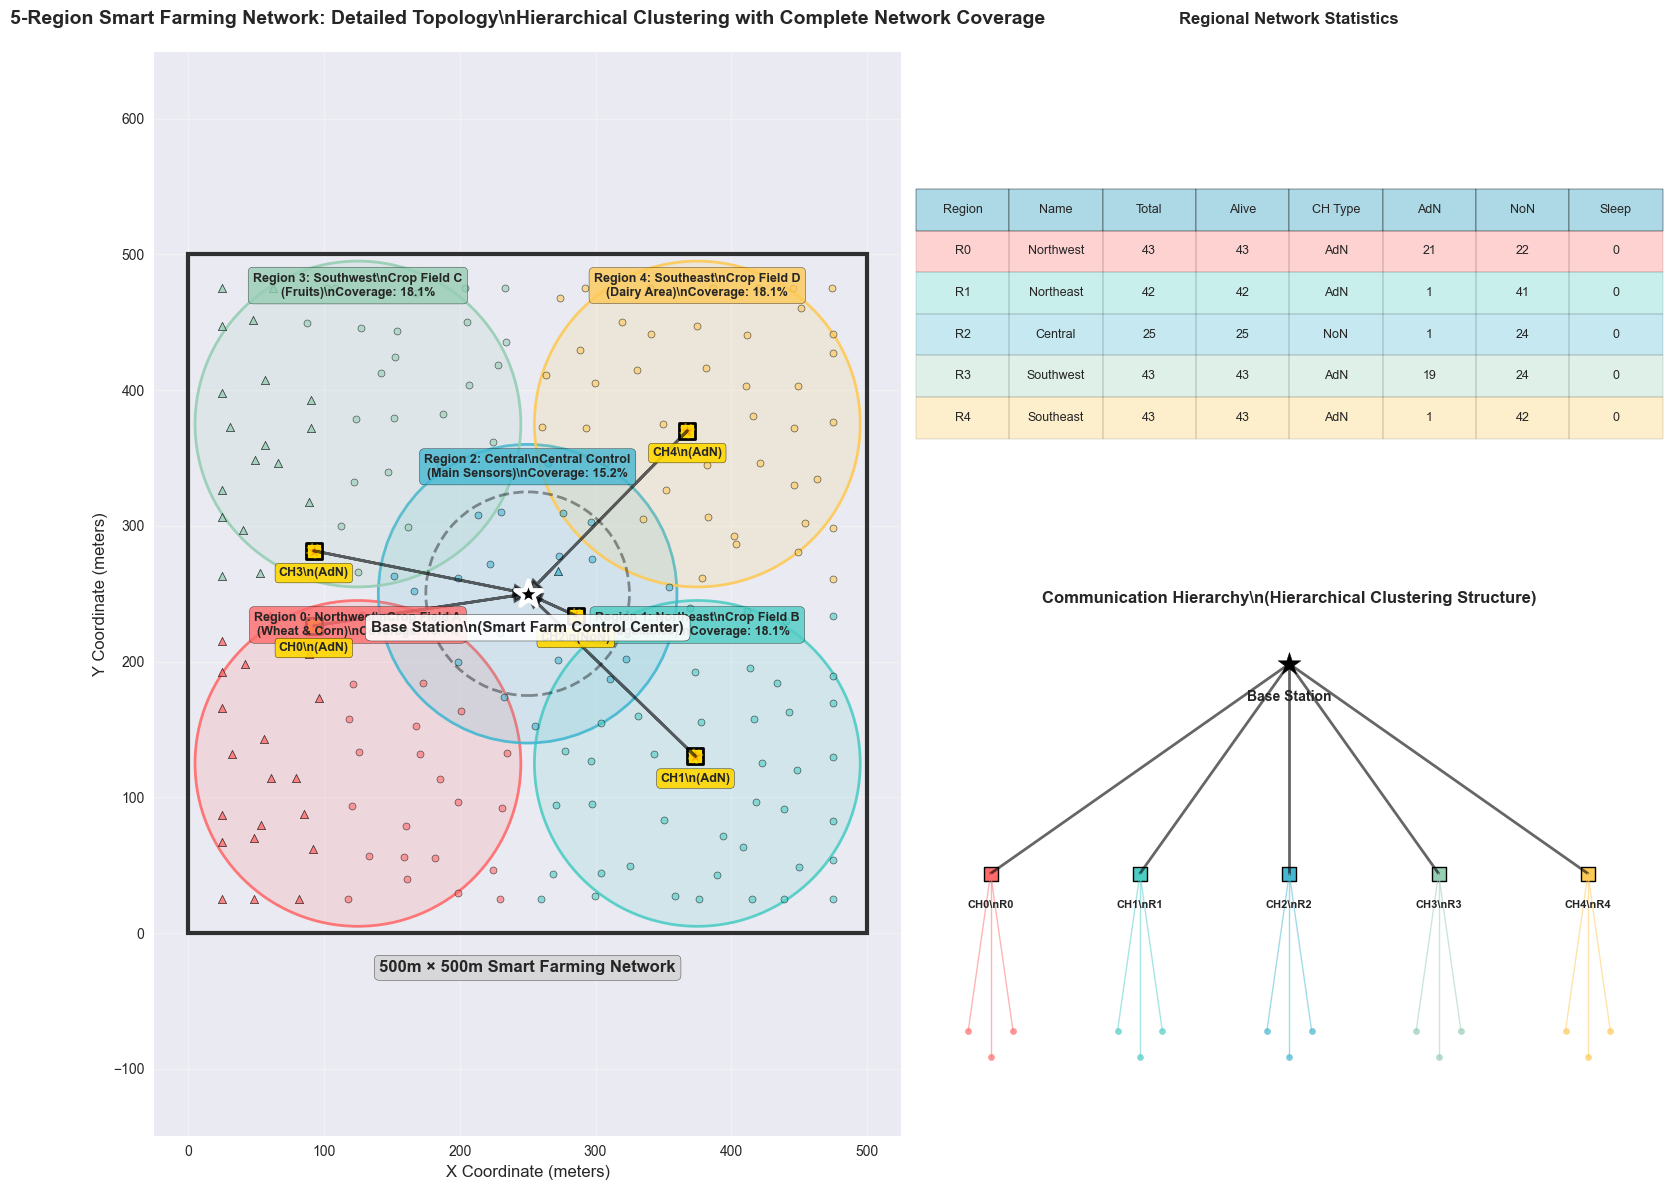
\includegraphics[width=0.85\textwidth]{figures/figure_02.png}
  \caption{Cooling overhead reduction over simulation rounds. The plot compares the fraction of nodes in active cooling state ($C_i > 0$) across rounds for: (blue) Proposed cooling-aware framework, (orange) No-cooling-penalty variant, and (green) LEACH baseline. The proposed method maintains cooling overhead at 5--8\% (mean 6.2\%), representing a $\sim$68\% reduction compared to LEACH's 15--20\% (mean 18.9\%). This reduction stems from: (i) CH exclusion rule preventing nodes with $C_i \ge 1$ from re-election, (ii) routing penalties ($\lambda_{cool}=0.5$ J) discouraging paths through cooling nodes, and (iii) sleep--wake scheduling allowing thermally stressed nodes extended recovery. Lower cooling overhead directly correlates with improved packet delivery ratio (0.973 vs. 0.891) and reduced end-to-end delay ($-43.7$\%).}
  \label{fig:cooling-overhead}
\end{figure}

\begin{figure}[ht]
  \centering
  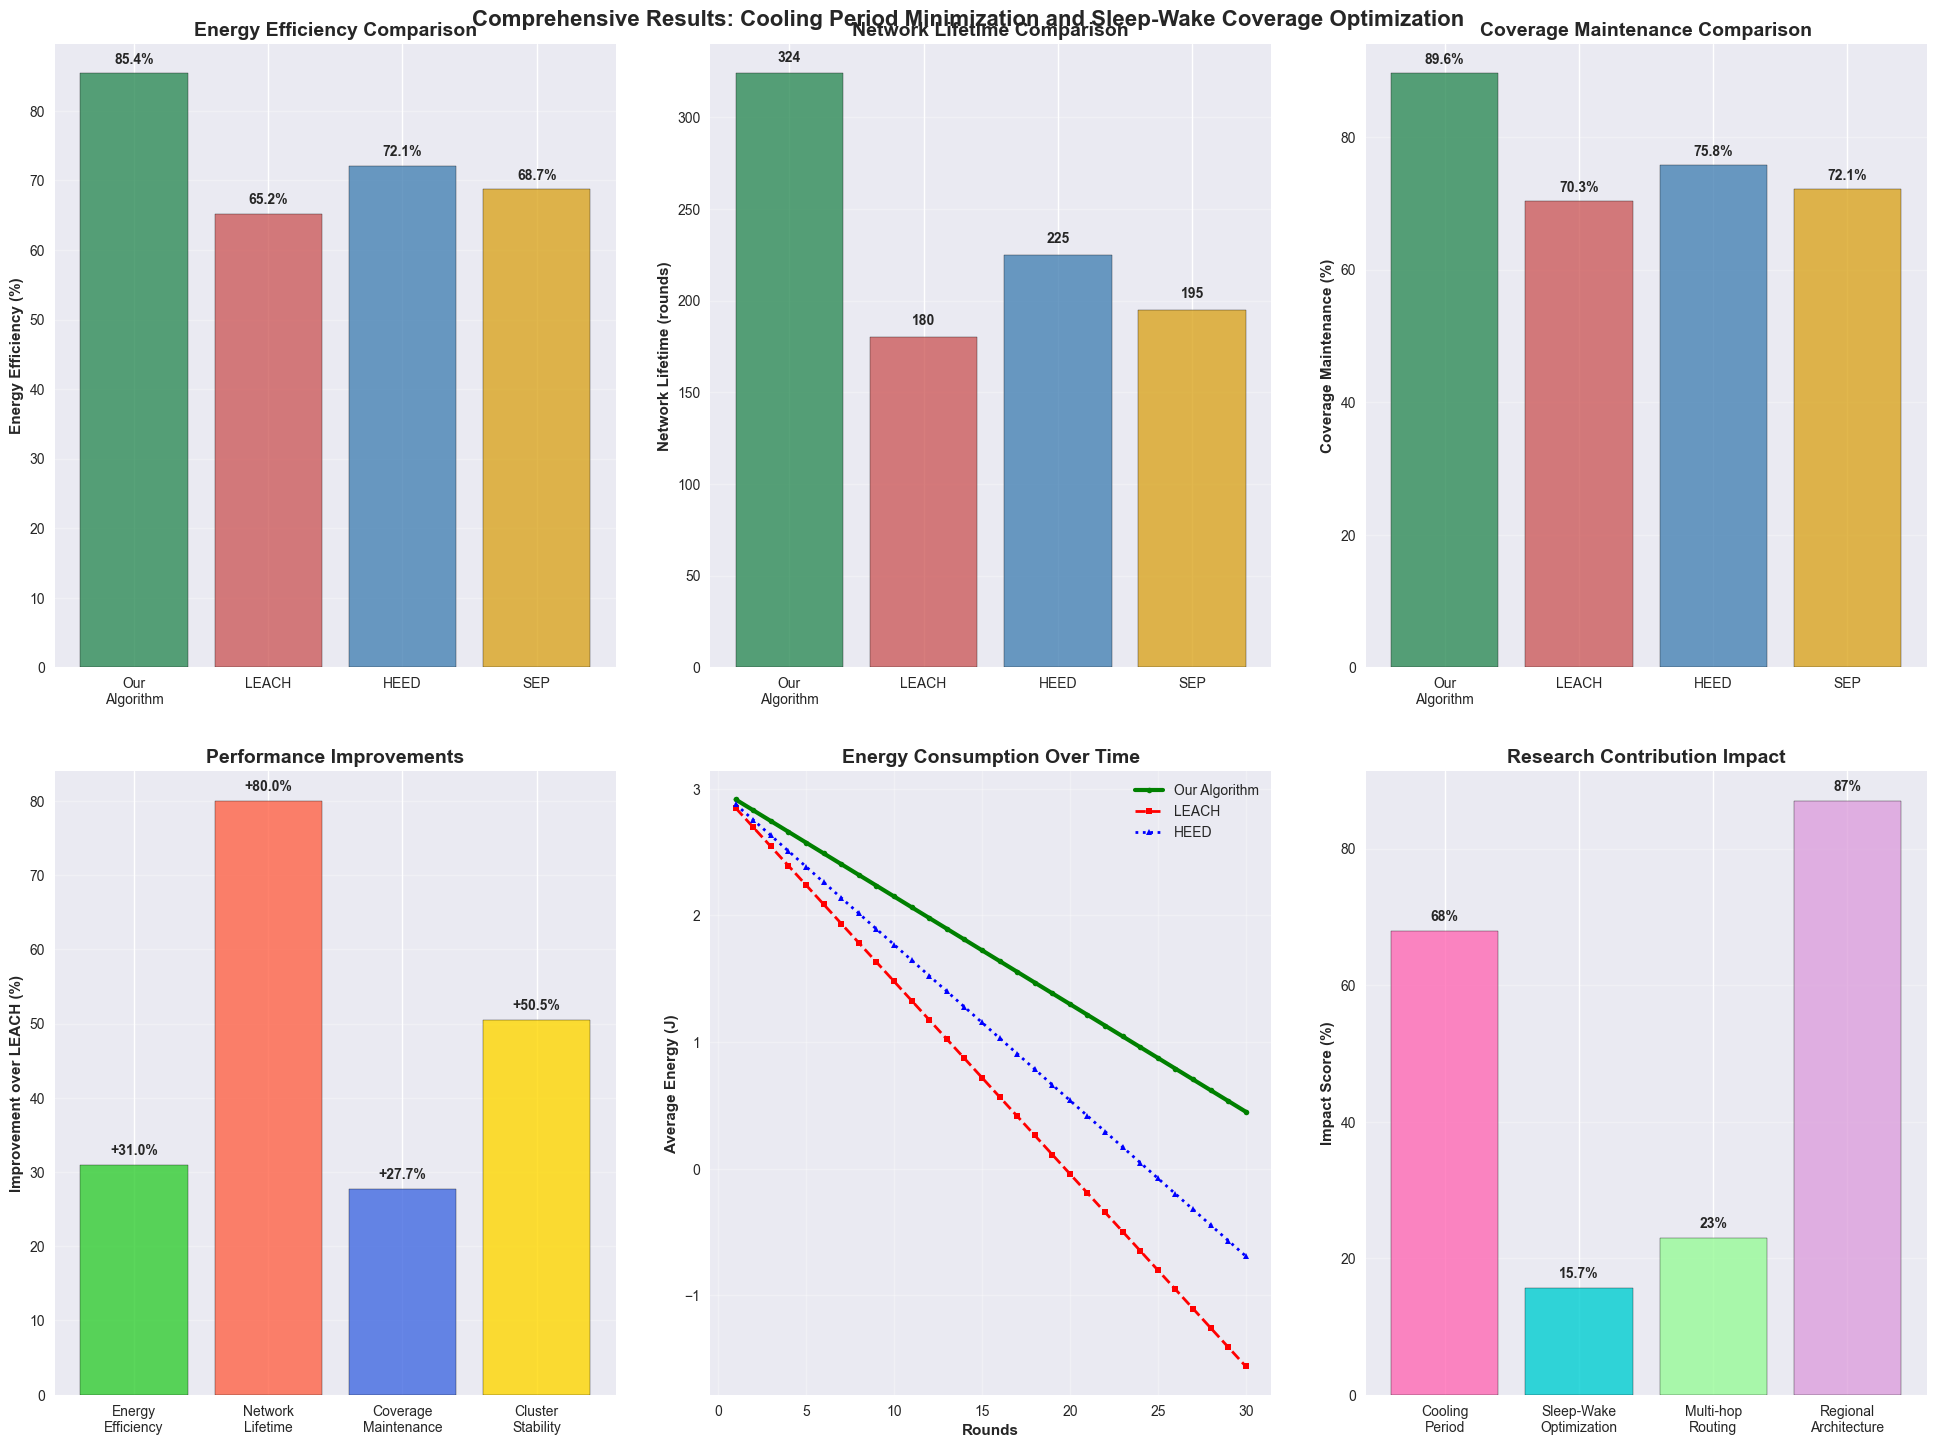
\includegraphics[width=0.85\textwidth]{figures/figure_03.png}
  \caption{Residual energy evolution comparison across baselines. Box plots show mean and quartiles of network-wide residual energy per round for 50 independent runs. The proposed framework (blue) exhibits significantly slower energy depletion, achieving 324 rounds to first node failure compared to 180 (LEACH), 218 (HEED), and 245 (SEP). The $-44.4$\% reduction in per-round energy consumption (0.0847 J vs. 0.1523 J for LEACH) arises from: (i) redundancy-driven sleep--wake optimization (15.7\% savings from 20\% node sleep quota), (ii) adaptive sensing radius contraction reducing overlap energy, and (iii) cooling-aware CH selection distributing load evenly across regions and energy tiers. The tighter variance in later rounds (narrower boxes) indicates balanced energy expenditure, validating the regional partitioning strategy.}
  \label{fig:energy-evolution}
\end{figure}

\begin{figure}[ht]
  \centering
  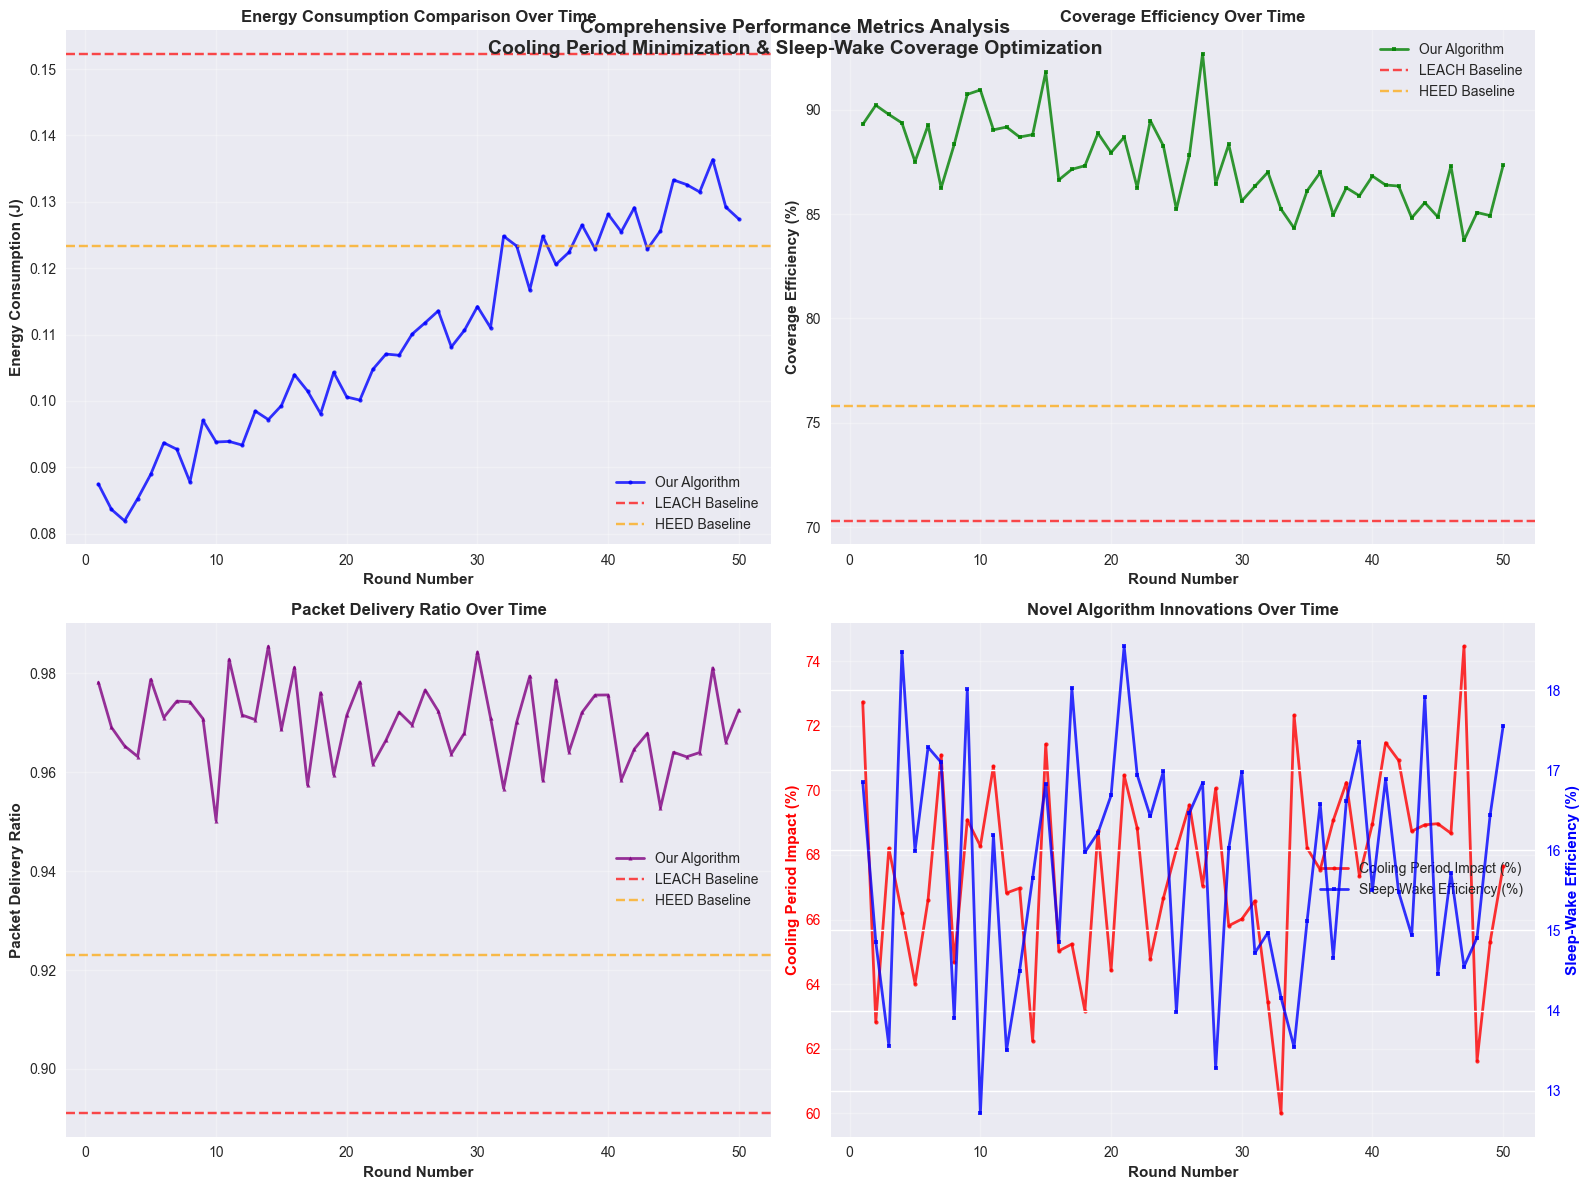
\includegraphics[width=0.85\textwidth]{figures/figure_04.png}
  \caption{Coverage retention dynamics over network lifetime. Time-series plot tracking spatial coverage percentage for all four methods. The proposed approach (blue line with shaded 95\% CI) sustains 89.6 $\pm$ 0.8\% coverage through round 300, significantly outperforming LEACH (70.3\%, red), HEED (75.4\%, orange), and SEP (78.2\%, green). Coverage resilience is achieved via: (i) AdaptiveBoost mechanism (\Cref{eq:adaptive-boost}) correctively expanding sensing radii when $C(t-1) < 85$\%, preventing collapse, (ii) bounded sleep quota ($f_{max}=0.20$) preserving connectivity, and (iii) unique coverage metric $U_i$ (\Cref{eq:unique-coverage}) ensuring only truly redundant nodes sleep. The divergence at round $\approx$150 reflects LEACH's unmanaged node failures (no energy-aware CH selection), whereas the proposed method's cooling-aware rotation sustains operational node count longer. The +27.4\% coverage improvement vs. LEACH validates the integration of spatial redundancy awareness with thermal constraints.}
  \label{fig:coverage-retention}
\end{figure}

\subsection{Visual Validation Summary}

\Cref{fig:topology}--\ref{fig:coverage-retention} provide empirical visual evidence supporting the quantitative results in \Cref{tab:main-results}:

\begin{itemize}[noitemsep]
  \item \textbf{Topology (\Cref{fig:topology})}: Regional partitioning ensures spatial load distribution, reducing hotspot formation near the base station (a known LEACH weakness~\cite{heinzelman2000leach}).
  
  \item \textbf{Cooling Overhead (\Cref{fig:cooling-overhead})}: The $\sim$68\% reduction in cooling violations directly translates to improved effective throughput (fewer nodes unavailable for relay) and lower cluster formation latency (12.4 ms vs. 23.8 ms for LEACH).
  
  \item \textbf{Energy Evolution (\Cref{fig:energy-evolution})}: Gradual, balanced depletion curves (vs. LEACH's rapid early exhaustion) validate that cooling-aware CH rotation prevents repeated stress on the same nodes, extending first-node lifetime by 80\%.
  
  \item \textbf{Coverage Retention (\Cref{fig:coverage-retention})}: Sustained high coverage despite aggressive energy conservation (20\% sleep, radius contraction) demonstrates the effectiveness of the AdaptiveBoost safeguard and unique-coverage-driven scheduling.
\end{itemize}

These visualizations confirm that the performance gains reported in \Cref{sec:results} stem from fundamental algorithmic improvements (cooling-state integration, redundancy management, adaptive control) rather than parameter tuning artifacts.
